\documentclass{article}
\usepackage{qilin}
\tikzstyle{process} = [rectangle, rounded corners, minimum width=1.5cm, minimum height=0.5cm,align=center, draw=black, fill=gray!30, auto]
\title{\vspace{-15mm}AER372: Easy Solution to Pendulum on a Cart \vspace{-6mm}}
\author{QiLin Xue}
\date{}
\usepackage{mathrsfs}
\usetikzlibrary{arrows}
\usepackage{stmaryrd}
\usepackage{accents}
\newcommand{\ubar}[1]{\underaccent{\bar}{#1}}
\usepackage{pgfplots}

\begin{document}

\maketitle
\vspace{-4mm}
\section*{Problem}
\vspace{-2mm}
Consider a freely rotating rigid pendulum of mass $m_p$, length $2\ell$ and moment of inertia $I$ about its center of mass, attached to a cart of mass $m_t.$ The cart is being pushed with a force $u(t)$ and the damping constant is $b.$
\begin{center}
    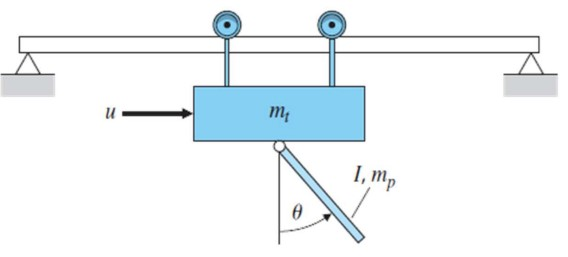
\includegraphics[width=0.4\textwidth]{w3_tut1.jpg}
\end{center}
\section*{Simple Solution}
\vspace{-2mm}
We can describe the system by the coordinates $(x,\theta).$ We apply d'Alambert's Principle. Specifically, we change into an accelerating frame of reference by adding a force $-m_t\ddot{x}$ to all bodies, such that $m_t$ is stationary. The free body diagram now looks like this, where we have neglected internal forces:
\begin{center}
    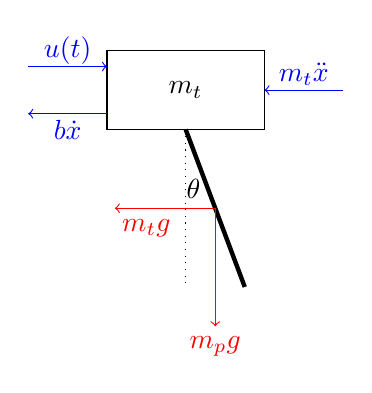
\begin{tikzpicture}
        % Draw rectangle from (0,0) to (0,2) and label the center 
        \draw (0,0) rectangle (2,1);
        \node at (1,0.5) {$m_t$};

        % Force vector
        \draw[blue, ->] (-1,0.8) -- (0,0.8);
        \node[blue] at (-0.5,1) {$u(t)$};

        \draw[blue, <-] (-1,0.2) -- (0,0.2);
        \node[blue] at (-0.5,0) {$b\dot{x}$};

        \draw[blue, ->] (3,0.5) -- (2,0.5);
        \node[blue] at (2.5,0.7) {$m_t\ddot{x}$};

        % Draw thick line from (0.5,0) to (0.75,-1.2)
        \draw[ultra thick] (1,0) -- (1.75,-2);

        % Draw vertical dotted line and label theta
        \draw[dotted] (1,0) -- (1,-2);
        \node at (1.1,-0.75) {$\theta$};

        % mg vector on pendulum
        \draw[red, ->] (1.37500,-1) -- (1.37500,-2.5);
        \node[red] at (1.375,-2.75) {$m_p g$};

        % mtg vector on pendulum
        \draw[red, ->] (1.37500,-1) -- (0.1,-1);
        \node[red] at (0.5,-1.25) {$m_t g$};
    \end{tikzpicture}
\end{center}
Because the pivot point is stationary and because angles do not change under a different frame of reference, we can balance torques about the pivot, i.e. 
\begin{equation}
    \boxed{(I + m_p \ell^2)\ddot{\theta} = -m_pg \ell \sin\theta - m_tg\ell\cos\theta}.
\end{equation}
Next we consider forces on $m_t.$ Treating the block as its own system, we now have forces the pendulum exerts on the block. We can do this a clever way by applying d'Alambert's Principle a second time. The pendulum's acceleration can be decomposed into two components:
\begin{itemize}
    \item Component 1: radial acceleration towards the pivot point with magnitude $\ell \dot{\theta}^2.$
    \item Component 2: tangential acceleration, perpendicular to the pendulum, with magnitude $\ell \ddot{\theta}$
\end{itemize}
Then the free body diagram in this new accelerating reference frame is, (where we are able to combine $m_t$ and $m_p$ since they are both stationary)
\begin{center}
    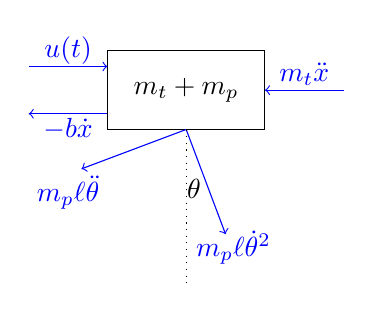
\begin{tikzpicture}
        % Draw rectangle from (0,0) to (0,2) and label the center 
        \draw (0,0) rectangle (2,1);
        \node at (1,0.5) {$m_t+m_p$};

        % Force vector
        \draw[blue, ->] (-1,0.8) -- (0,0.8);
        \node[blue] at (-0.5,1) {$u(t)$};

        \draw[blue, <-] (-1,0.2) -- (0,0.2);
        \node[blue] at (-0.5,0) {$-b\dot{x}$};

        \draw[blue, ->] (3,0.5) -- (2,0.5);
        \node[blue] at (2.5,0.7) {$m_t\ddot{x}$};

        % Draw thick line from (0.5,0) to (0.75,-1.2)
        \draw[blue,->] (1,0) -- (1.5,-1.33);
        \node[blue] at (1.6,-1.5) {$m_p\ell \dot{\theta}^2$};

        % Draw tangential vector perpendicular to line above
        \draw[blue,->] (1,0) -- (-0.33,-0.5);
        \node[blue] at (-0.5,-0.8) {$m_p\ell \ddot{\theta}$};

        % Draw vertical dotted line and label theta
        \draw[dotted] (1,0) -- (1,-2);
        \node at (1.1,-0.75) {$\theta$};

        % % mg vector on pendulum
        % \draw[red, ->] (1.37500,-1) -- (1.37500,-2.5);
        % \node[red] at (1.375,-2.75) {$m_p g$};

        % % mtg vector on pendulum
        % \draw[red, ->] (1.37500,-1) -- (0.1,-1);
        % \node[red] at (0.5,-1.25) {$m_t g$};
    \end{tikzpicture}
\end{center}
This is static, so the net force is zero. Decomposing everything to be in the $x$-direction, we have:
\begin{equation}
    \boxed{m_t\ddot{x} = u(t) - b\dot{x} + m_p\ell \ddot{\theta}\cos\theta - m_p\ell \dot{\theta}^2\sin\theta}.
\end{equation}
\item d 
\item \begin{enumerate}[label=(\alph*)]
    \item If we have repeated roots, then we can factor
    \begin{equation}
        H(s) = \frac{\omega_n^2}{(s+\omega_n)^2},
    \end{equation}
    i.e. $\zeta = 1.$
\end{enumerate}
\end{enumerate}
\end{document}